\chapter{Estudos de Caso}
\label{cap:estudos-de-caso}

%Explicar o porque de cada cenário
%Detalhar implementação e experimentos realizados:

Foram realizados dois experimentos como estudo de caso, utilizando as duas implementação apresentadas no capítulo anterior, sendo elas os cenários de estacionamento e tráfego de carros inteligente.
Através desses dois experimentos pudemos validar a proposta de solução apresentada para construção de um ambiente simulado de experimentação para plataformas de Cidades Inteligentes.
Foi possível exercitar as principais funcionalidades necessárias para a realização de experimentos desse tipo, através da integração do InterSCSimulator e a plataforma InterSCity.

Os cenários simulados em cada experimento e seus respectivos resultados serão apresentados nas seções a seguir.
E ao final, realizaremos uma análise crítica sobre os resultados obtidos nesses estudos de caso, apontando possíveis melhorias a serem feitas.

\section{Estacionamento Inteligente}
\label{sec:exp_smart_parking}

Como apresentado na Seção \ref{sec:smart_parking}, nesse cenário de Cidades Inteligentes simulamos a utilização de um aplicativo móvel, por parte dos motoristas de carros, para facilitar o encontro de
vagas de estacionamento disponíveis próximas do seu destino final.
Esse aplicativo poderia evitar alguns transtornos para os motoristas na árdua missão de estacionar seus carros no centro das grandes metrópoles, por exemplo.

Nesse experimento, tentamos verificar a escalabilidade dos microsserviços envolvidos da plataforma InterSCity, por isso utilizamos dados reais de uma das maiores megalópoles do mundo: São Paulo.
Dados abertos da cidade de São Paulo foram utilizados para a definição do cenário de simulação do ambiente integrado.
Utilizamos dados extraídos da pesquida OD (Origem-Destino) realizada pela Companhia de Metrô da cidade de São Paulo e do OpenStreet Maps para a definição de cenário.
A seguir, esses dados, bem como suas fontes, utilizados na configuração do experimento serão detalhados:

\begin{itemize}
    \item \textbf{Pesquisa Origem-Destino (OD)}: criamos as viagens de carro simuladas com base na pesquisa OD realizada pela Companhia de Metrô de São Paulo em 2007.
        \footnote{Pesquisa Origem-Destino - http://goo.gl/Te2SX7.}
        Essa pesquisa descreve as viagens de 200.000 pessoas e extrapola os dados para toda a população da cidade.
        A pesquisa inclui informações sobre a origem, o destino, o modo de transporte e a hora de partida.
        Esses dados foram utilizados para definir o comportamento dos agentes do tipo carro na simulação.
        Para gerar a carga de trabalho para a plataforma, simulamos o tráfego em São Paulo durante um dos horário de pico, das 5h40 às 8h40.
        Na pesquisa OD, há 492.976 carros que começam suas viagens durante o intervalo de tempo considerado.

    \item \textbf{OpenStreet Maps}: para criar o grafo viário da cidade de São Paulo usado na simulação, usamos o mapa do OpenStreet Maps.
        Este mapa contém todas as ruas e junções da cidade, em conjunto com um vasto número de atributos, como comprimento, capacidade e velocidade limite.
        Tais informações são usadas pelo simulador para definir as rotas percorridas pelos carros durante a realização de suas viagens, bem como simular o impacto do tráfego na velocidade dos carros.

    \item \textbf{Vagas de Estacionamento}: criamos as vagas de estacionamento na simulação baseado nos dados obtidos através do OpenStreet Maps e do Zona Azul
        \footnote{http://www.cetsp.com.br/consultas/zona-azul/mapa-zona-azul/mapa-zona-azul.aspx}
        (serviço de estacionamento rotativo da cidade de São Paulo).
\end{itemize}

Nas Figuras \ref{fig:map-spots-distribution} e \ref{fig:map-destinations-distribution}, são apresentadas as distribuições das vagas de estacionamento e destinos de viagens de carros respectivamente,
utilizadas nesse experimento.
Os destinos apresentados na Figura \ref{fig:map-destinations-distribution}, são referentes a todas as viagens realizadas no decorrer de toda a simulação.
É importante notar que a distribuição das vagas de estacionamento baseado nesses dados reais está mais concentrada no centro da cidade do que os destinos das viagens.
Isso pode levar a situaçãoes onde o agente do tipo carro pode realizar mais de três tentativas de busca de vagas disponíveis e ainda sim não conseguir estacionar.
Nesse caso, o usuário do aplicativo pararia de utilizá-lo e o agente do tipo carro terminaria sua execução, como apresentado na Seção \ref{sec:smart_parking}.

\begin{figure}[!ht]
    \centering
    \includegraphics[width=8cm]{figuras/mapa_vagas.pdf}
    \caption{Mapa de calor com a distribuição das vagas de estacionamento utilizadas no experimento.}
    \label{fig:map-spots-distribution}
\end{figure}

\begin{figure}[!ht]
    \centering
    \includegraphics[width=8cm]{figuras/mapa_viagens.pdf}
    \caption{Mapa de calor com a distribuição dos destinos de viagens de carro utilizadas no experimento.}
    \label{fig:map-destinations-distribution}
\end{figure}

Tendo ideia do contexto e dos dados a serem utilizados nesse cenário experimental, os passos a seguir foram executados no decorrer deste experimento:

\begin{enumerate}
    \item Executar uma instância em modo de produção da plataforma InterSCity em um ambiente de núvem. O ambiente de núvem proporciona maior flexibilidade para escalar os microsserviços em tempo
        de execução.

    \item Habilitar mecanismo de escala automática (\textit{auto-scaling}) para os microsserviços da plataforma baseado na variação de carga de trabalho.

    \item Configuração do simulador em um ambiente isolado da plataforma. Assim, o gasto de recursos computacionais do simulador não interfere no uso da plataforma.

    \item Realizar a simulação do cenário de estacionamento inteligente.

    \item Monitorar a performance e o uso de recursos da plataforma durante toda a simulação.

    \item Analizar os resultados obtidos.
\end{enumerate}

Então, inicialmente, foi necessário a configuração de ambas as ferramentas em conjunto com seu componente de integração em um ambiente de núvem.
Os microsserviços da plataforma InterSCity, o simulador InterSCSimulator e ferramentas auxiliares foram implantados na forma de \textit{containers} Docker \footnote{https://www.docker.com/}.
Utilizamos a infraestrutura provida pelo Google Cloud Platform (GCP) \footnote{https://cloud.google.com/} para a realização do experimento, sendo esse o ambiente ideal para a execução da plataforma
InteSCity, como visto na Seção \ref{sec:interscity}.
No contexto do GCP, fizemos bastante uso do Google Kubernetes Engine (GKE), sendo esse um serviço que provê um ambiente gerenciado e de produção para implantação de \textit{containers} de
aplicações.
O Kubernetes foi utilizado principalemte para automatizar a reinicialização, a replicação e dimensionamento do número de \textit{containers}.
Além disso, o kubernetes traz uma vantagem para a reprodutibilidade do experimento que é a especificação da infraestrutura como código, garantindo a correta aplicação das regras de implantação.
Todo o código fonte utilizado para a realização desse experimento está disponível em repositório aberto na web \footnote{https://github.com/LSS-USP/interscity-k8s-experiment}.

Nós dividimos o \textit{cluster} utilizado em cinco diferentes \textit{pools} de máquinas virtuais para que o Kubernetes pudesse gerenciar os \textit{containers} no contexto apropriado.
Na Figura \ref{fig:node-pools}, são apresentados os \textit{pools} de nós, contendo o número e o tipo de máquinas virtuais utilizadas por cada um no GCP
\footnote{https://cloud.google.com/compute/docs/machine-types}.
O \textit{pool} da plataforma possui 25 máquinas do tipo n1-standard-2 (2 CPUs virtuais e 7.5GB memória) e executa os microsserviços da plataforma InterSCity.
Existem três conjuntos de nós adicionais (representados em azul) compostos por n1-high-2 máquinas (2 CPUs virtuais e 13GB de memória), que executam os serviços de suporte da plataforma InterSCity.
Ambos MongoDB e PostgreSQL têm 5 nós sendo executados de maneira distribuída, instâncias tolerantes a falha de seus respectivos sistemas de banco de dados.
O RabbitMQ possui uma máquina dedicada em um \textit{pool} isolado.
MongoDB é implementado usando a estratégia de conjunto de réplicas (\textit{replica set}), onde operações de leitura são distribuídas entre nós secundários (escravos), e operações de escrita são
sempre executadas no nó primário (mestre).
A mesma estratégia é adotada na implantação do PostgreSQL, para otimizar as operações de leitura executadas pelo \textit{Resource Catalog}.
Finalmente, o InterSCSimulator é executado em sua própria máquina n1-highmem-16 (16 CPUs virtuais e 104 GB de memória), isoladas do resto do serviços.

\begin{figure}[ht]
	\centering
	\includegraphics[width=0.7\textwidth]{figuras/node-pools.png}
    \caption{Configuração do \textit{cluster} para o experimento.}
	\label{fig:node-pools}
\end{figure}


Para o conjunto de nós da plataforma, o Kubernetes pode programar a implantação de vários \textit{containers} para a mesma máquina, dependendo da disponibilidade de recursos computacionais.
A distribuição de \textit{containers} nos 25 nós pode diferir de uma rodada do experimento para a outra, e é uma variável que nós não controlamos durante o experimento.
Para avaliar o impacto de tais variações na análise, realizamos 15 rodadas deste experimento e verificamos a variabilidade dos resultados.

Como estávamos interessados em avaliar a escalabilidade da plataforma considerando um cenário de Cidades Inteligentes com uma carga de trabalho variável, usamos dimensionamento automático
(\textit{auto-scaling}) para o \textit{Resource Catalog}, \textit{Resource Discovery}, \textit{Data Collector}, já que eles são projetados para escalar horizontalmente.
Para este propósito, especificamos um valor alvo de 60\% de uso da CPU para cada um desses serviços, permitindo que o sistema aumente ou diminua o número de \textit{containers} por serviço baseado nisso.
O sistema balanceia a carga de trabalho para corresponder ao valor alvo de uso da CPU, considerando o uso médio da CPU dos \textit{containers} em execução, que é medido a cada 30 segundos.
Inicialmente, cada serviço tem quatro \textit{containers}, que é definido como o número mínimo de \textit{containers} em execução.
Este número pode aumentar a medida que os recursos computacionais ficarem disponíveis no \textit{pool} de nós da plataforma.
Os \textit{containers} são executados por trás de um serviço de balanceamento de carga.

Embora possamos nos beneficiar das propriedades de elasticidade do GCP, adicionando e removendo automaticamente nós ao \textit{cluster} através da sua funcionalidade de dimensionamento automático,
isso introduziria outro nível de incerteza em nosso experimento, já que na nossa experiência o tempo levado para criar novas máquinas virtuais pode variar consideravelmente.
Sabendo disso, criamos todos os nós previamente, antes de iniciar o experimento, mantendo-os em execução ao longo de todo experimento.

Como dito anteriormente, executamos 15 rodadas de experimentos, onde cada uma durou 3h, correspondendo ao horário de pico da manhã da cidade de São Paulo descrito no início desta seção.
Na Figura \ref{fig:workload}, podemos ver a carga de trabalho média gerada pela simulação durante todo o experimento e o seu desvio padrão (linhas pretas no topo de cada barra).
Vale notar que nos primeiros 80 minutos de simulação, temos um crescimento constante da carga de trabalho.
No intervalo aproximado de uma hora, entre 60 e 120 minutos, observamos o período de maior carga do experimento, considerando que o pico máximo de requisições ocorre após 80 minutos, correspondendo a mais
de 113.000 requisições em 10 minutos.
No total, mais de um milhão de requisições foram realizadas para a plataforma durante o tempo de experimento.
Considerando que para responder cada uma dessas requisições requer um conjunto complexo de operações com várias etapas internas, isso se traduz em uma carga computacional muito alta.

\begin{figure}[ht]
	\centering
	\includegraphics[width=0.7\textwidth]{figuras/workload.png}
    \caption{Média da carga de trabalho gerada pelo InterSCSimulator no decorrer do experimento.}
	\label{fig:workload}
\end{figure}

A Figura \ref{fig:auto-scaling} mostra a criação e destruição dinâmica de \textit{containers} da plataforma InterSCity devido à aplicação da estratégia de dimensionamento automático em uma única rodada
do experimento.
A replicação inicial das instâncias de Kong (balaceador de carga) foi suficiente para suportar toda a carga de trabalho durante todo o experimento, já que ele executa apenas a tarefa de baixa latência
de encaminhar as requisições de entrada aos microsserviços apropriados.
Por sua vez, os três microsserviços da plataforma, que são responsáveis por processar as requisições de fato, foram replicados de acordo com o aumento da carga de trabalho.
Portanto, o número de \textit{containers} para esses serviços variou de 4 a 25.
É importante mencionar que o mecanismo de elasticidade da plataforma InterSCity também reduziu o número de \textit{containers} à medida que a demanda diminuiu.
Como pode ser visto na Figura \ref{fig:auto-scaling}, dentre os microsserviços da plataforma, o \textit{Data Collector} foi o microsserviço que consumiu menos tempo de CPU.

\begin{figure}[ht]
	\centering
	\includegraphics[width=0.7\textwidth]{figuras/auto-scaling.png}
    \caption{Dimensionamento automáticos dos microsserviços da plataforma InterSCity.}
	\label{fig:auto-scaling}
\end{figure}


A Figura \ref{fig:throughput} mostra a taxa de vazão (\textit{throughput}) média da plataforma InterSCity ao longo da duração do experimento.
A taxa de vazão é definida como a taxa de respostas bem sucedidas recebidas pelo componente de integração.
O resultado indica que a taxa de vazão corresponde de perto a carga de trabalho gerada, como pode ser visto comparando as Figuras \ref{fig:workload} e \ref{fig:throughput}.
Apesar das variações no comportamento dos condutores de carros ao longo do experimento, a plataforma foi capaz de lidar com a demanda variável graças a sua escalabilidade e funcionalidade de dimensionamento
automático, descritos na Seção \ref{sec:interscity}.
No entanto, devemos mencionar que a taxa de vazão não correspondeu exatamente à carga de trabalho gerada, pois algumas requisições falharam, representando quase 0,6\% de todas as requisições em média.
As requisições com falha incluem aquelas que tiveram respostas com um código de erro HTTP, bem como aquelas que não foram concluídos devido a recusa de conexão ou \textit{timeout}.
Todavia, nós consideramos que ser capaz de lidar com mais de 99,5\% das requisições sob alta carga é satisfatório; um usuário típico perceberia uma falha a cada 200 requisições, o que é muito bom para
este tipo de aplicação de Cidades Inteligentes em tempo real.

\begin{figure}[ht]
	\centering
	\includegraphics[width=0.7\textwidth]{figuras/throughput.png}
    \caption{Taxa de vazão (\textit{throughput}) média da platafora InterSCity.}
	\label{fig:throughput}
\end{figure}


Outro aspecto fundamental da avaliação de um sistema é analisar o desempenho da plataforma para lidar com requisições de aplicação com uma carga de trabalho variável.
A este respeito, estamos interessados principalmente em analisar a degradação do desempenho e verificar se a plataforma está sendo dimensionada adequadamente para atender seus clientes dentro de tempos
de resposta aceitáveis.
Para tanto, coletamos o tempo de resposta do ponto de vista do cliente, como mostrado Figura \ref{fig:responsetime}.
Durante a maior parte do experimento, a plataforma foi capaz de responder em menos de um segundo.
No entanto, diferente da taxa de vazão, o impacto do maior período de demanda no tempo de resposta observado é perceptível, uma vez que, durante um intervalo curto (após 110 minutos de execução),
o tempo médio de resposta foi maior que 1 segundo.
O tempo de resposta voltou para 500 milisegundos depois disso.
Entretanto, podemos ver que mesmo em períodos de alta carga, o tempo de resposta foi mantido abaixo de 2 segundos, o que é um resultado muito bom para este tipo de aplicação.

\begin{figure}[ht]
	\centering
	\includegraphics[width=0.7\textwidth]{figuras/response_time_mean.png}
    \caption{Tempo de resposta médio da platafora InterSCity.}
	\label{fig:responsetime}
\end{figure}


Devemos ter em mente que a distribuição de \textit{containers} nos nós disponíveis podem impactar o tempo de resposta, pois vários \textit{containers} podem competir por recursos computacionais se estiverem
sendo executados na mesma máquina.
Além disso, embora o sistema realize a tarefa de dimensionamento automático a cada 30 segundos, não temos controle sobre o tempo que leva para um \textit{container} ser criado, implantado e ficar pronto
para receber novas requisições.
Por outro lado, essa distribuição também pode introduzir um efeito benéfico devido a possível implantação de serviços que constantemente interagem uns com os outros na mesma máquina, reduzindo a latência
de rede e imprevisibilidade.

\section{Tráfego de Carros Inteligente}

Neste segundo experimento, simulamos o trânsito de uma cidade, e através de uma aplicação de detecção de anomalias em vias (variação da velocidade média dos carros bem acima do usual),
atuamos em Placas de Mensagens Variadas (PMV) alertando os motoristas desses trechos problemáticos para que os mesmos fossem evitados.
Essa aplicação de detecção de anomalias em vias foi implementada utilizando o serviço de processamento de dados da plataforma InterSCity que está em desenvolvimento.

Esse experimento consistiu em três etapas.
Com discutido na Seção \ref{sec:smart_traffic}, limiares (\textit{thresholds}) de velocidade média para cada trecho de via em cada horário do dia deveriam ser definidos.
Portanto, a primeira etapa consistiu na simulação do trânsito da cidade sem nenhum evento de fechamento de via, ou seja, o trânsito normal da cidade.
Com isso, a aplicação de detecção de anomalias foi capaz de, com os dados de posicionamento de carros enviados a cada ciclo de execução, definir esses tais limiares.
Já a segunda etapa, consistiu em simular o trânsito de carros na cidade com alguns eventos de fechamento de vias (representando ruas alagadas e acidentes de carro por exemplo).
Nessa etapa, simulamos o comportamento caótico visto nas grandes cidades, onde vias são interditadas e interferem diretamente no tráfego dos carros.
Na última etapa, simulamos o mesmo comportamento da segunda etapa, mas adicionamos as PMVs para auxiliar os condutores de carros a contornar essas situações.
Tendo em vista que os limiares já haviam sido definidos, a aplicação, sem ter conhecimento prévio dessas vias fechadas, detectava automaticamente esses trechos e notificava os motoristas através da
atualização de mensagens nas PMVs.
O objetivo dessas três etapas era verificar o impacto do uso de PMVs no tempo de duração médio das viagens de carro em situações de incidentes que inviabilizam a utilização de certas vias em uma cidade.

Para verificar o bom funcionamento desse cenário no ambiente simulado, dividimos esse experimento em dois.
Na primeira parte, realizamos um experimento numa escala menor e com dados fictícios, visando meramente a validação do comportamento esperado e interação entre os componentes.
Na segunda parte, utilizamos dados abertos da cidade de São Paulo, aumentando a escala do experimento e se aproximando de um cenário mais realista.
O código fonte para a execução do experimento e a análise apresentada aqui nesta seção estão disponível em nosso repositório aberto
\footnote{https://github.com/LSS-USP/pmv\_experiment/blob/master/Analysis.ipynb}.

\subsection{Validação}

Nesse experimento inicial de validação, as três etapas se deram da seguinte forma com o que diz respeito a número de eventos de fechamento de via e PMVs:

\begin{enumerate}
    \item Sem eventos de fechamento de via e sem PMVs

    \item Com um evento de fechamento de via e sem PMVs

    \item Com um evento de fechamento de via e uma PMV
\end{enumerate}

Foram executadas 20 iterações de cada uma das etapas, onde em cada iteração foram 10 minutos de simulação.
Em todas as etapas, utilizamos um grafo com 8 vértices e 16 arestas, como pode ser visto na Figura \ref{fig:mapa_validacao}.
O grafo é direcionado, onde cada aresta na verdade representa duas, sendo uma entrando e outra saíndo de seus vértices, ou seja, simbolizam vias de mão dupla.

\begin{figure}[ht]
	\centering
	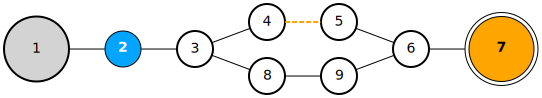
\includegraphics[width=\textwidth]{figuras/mapa_validacao.png}
	\caption{Mapa viário da cidade utilizado para validação.}
	\label{fig:mapa_validacao}
\end{figure}

O grafo da Figura \ref{fig:mapa_validacao} retrata o mapa viário da cidade simulada da seguinte forma:

\begin{itemize}
    \item Os vértices representam início e/ou fim de uma ou mais ruas.

    \item As arestas representam as ruas da cidade.

    \item Todas as arestas possuem comprimento 1, por isso, a cada ciclo de simulação, caso seja possível, um carro percorre uma aresta.
\end{itemize}

Além disso, adotamos a seguinte forma para separar vértices e arestas que desempenham papel importante neste experimento:

\begin{itemize}
    \item A aresta pontilhada amarela representa a via da cidade que será fechada durante a simulação (essa aresta só será afetada nas etapas que posssuem tal evento).

    \item O vértice cinza representa a origem de todas as viagens simuladas.

    \item O vértice alaranjado representa o destino das viagens.

    \item O vértice azul representa o local da cidade que contém uma PMV que alertará os motoristas sobre possíveis anomalias nas vias.
\end{itemize}

Em todas as iterações de todas as etapas, simulamos um total de 100 viagens partindo do vértice 1 até o 7.
Como o intuito desse experimento era validar o comportamento da implementação do ambiente de experimentação como um todo, antes de apresentar os resultados obtidos, descrevemos o resultado esperado para
cada uma das etapas a seguir.

Na Figura \ref{fig:mapa_etapa1}, pode-se ver o caminho esperado que os carros percorresem na primeira etapa do experimento, onde não há a presença de eventos de fechamento de vias, nem muito menos PMV.
As arestas em \textbf{roxo} representam o trajeto do carro, as demais arestas não utilizadas forma removidas do grafo a título de legibilidade.
Note que ao chegar no vértice 3, ele sempre optará o caminho seguindo pelo vértice 4.
Isso acontece porque como mencionado anteriormente todas as arestas possuem o mesmo comprimento (ambos são um caminho mais curto até o destino), sendo o critério de desempate o menor índice.

\begin{figure}[ht]
	\centering
	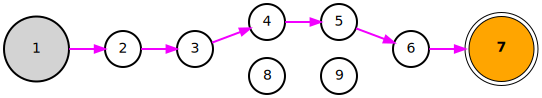
\includegraphics[width=\textwidth]{figuras/mapa_etapa1.png}
	\caption{Trajeto esperado da etapa 1 do experimento.}
	\label{fig:mapa_etapa1}
\end{figure}

Na Figura \ref{fig:mapa_etapa2}, o trajeto esperado para que o carro percorra na etapa 2 do experimento é apresentado.
Nessa etapa, temos uma via fechada, sendo ela entre os vétices 4 e 5, e nenhuma PMV para auxiliar os motoristas.
Em \textbf{roxo} podemos ver as arestas que serão percorridas inicialmente;
em cor \textbf{preta}, as arestas que faziam parte do caminho inicialmente calculado, mas que não foram percorridas devido ao fechamento da via (aresta tracejada);
e em cor \textbf{verde}, o caminho recalculado após se deparar com o fechamento de via no vértice 4.

\begin{figure}[ht]
	\centering
	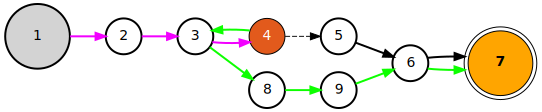
\includegraphics[width=\textwidth]{figuras/mapa_etapa2.png}
	\caption{Trajeto esperado da etapa 2 do experimento.}
	\label{fig:mapa_etapa2}
\end{figure}

Por fim, na Figura \ref{fig:mapa_etapa3}, temos a dinâmica esperada para a etapa 3, onde existe o fechamento da via, contudo a PMV se faz presente para notificar os condutores de veículos.
Mais uma vez, a via representada pela aresta 4 -> 5 é fechada, e a PMV é posicionada no vértice 2 representado em azul.
Utilizamos aqui a mesma notação anterior.
A aresta \textbf{roxa} representa o caminho inicialmente calculado e que foi percorrido;
as arestas \textbf{pretas} faziam parte do caminho inicial, mas nesse caso não forma percorridas devido ao fechamento da via e da PMV;
e as \textbf{verdes} simbolizam o novo caminho recalculado após o motorista ter sido notificado pela PMV do ocorrido.
Devido ao modelo implementado, ainda assim era esperado que alguns carros percorresem o fluxo apresentado na Figura \ref{fig:mapa_etapa2}, já que acreditamos que nem todos os motoristas que vissem
a notificação iriam de fato mudar o seu trajeto.

\begin{figure}[ht]
	\centering
	\includegraphics[width=\textwidth]{figuras/mapa_etapa3.png}
	\caption{Trajeto esperado da etapa 3 do experimento.}
	\label{fig:mapa_etapa3}
\end{figure}

As três etapas desse experimento foram realizadas em dois \textit{laptops} com 8 CPUs virtuais (1.80 GHz) e 8 GB de memória RAM.
Diferente do experimento apresentado na Seção \ref{sec:exp_smart_parking}, o foco desse experimento não é analisar o desempenho da plataforma, mas sim uma análise funcional. 
O passo a passo para execução desse experimento de validação foi o seguinte:

\begin{enumerate}
    \item Executar uma instância em modo de produção da plataforma InterSCity em um \textit{laptop}.

    \item Executar uma instância em modo de produção do simulador InterSCSimulator no outro \textit{laptop}.

    \item Configurar rede local entre os \textit{laptops}, conectados de maneira cabeada via ethernet.

    \item Realizar a simulação do cenário de tráfego de carros inteligente.

    \item Analizar os resultados obtidos ao final da simulação.
\end{enumerate}

A Figura \ref{fig:distancia_validacao}, apresenta o desvio padrão (no topo das barras) e a distância média percorrida pelos carros simulados nas três etapas deste experimento.
Segundo nossas hipóteses, esperávamos que no cenário sem evento de fechamento de via e sem PMV para notificar os motoristas percorressem 6 arestas, no cenário com evento e sem PMV percorressem 8 arestas
e no cenário com evento e PMV percorressem entre 6 e 8 arestas (alguns veículos ignoram as notificações).
Nossas hipóteses foram confirmadas, como pode ser visto no gráfico.

\begin{figure}[ht]
	\centering
	\includegraphics[width=.8\textwidth]{figuras/distancia_validacao.png}
	\caption{Média da distância percorrida pelos carros no experimento.}
	\label{fig:distancia_validacao}
\end{figure}

Uma análise semelhante foi realizada com a duração das viagens simuladas, como pode ser visto na Figura \ref{fig:duracao_validacao}.
O desvio padrão (no topo das barras) e a duração média das viagens simuladas nas três etapas do experimento são apresentados no gráfico.
Uma viagem dura sempre 2 ciclos de execução (criação e destruição do ator) mais o tempo utilizado para percorrer as arestas (uma aresta por ciclo de execução, já que possuem comprimento unitário)
e o recálculo de um caminho custa um ciclo.
Por isso, esperávamos que para o cenário sem evento de fechamento de via durasse 8 ciclos (2 pelo ciclo de vida + 6 arestas);
o cenário com evento e sem PMV para informar os motoristas durasse 11 ciclos (2 pelo ciclo de vida + 8 arestas + 1 pelo recálculo da rota);
e o cenário com evento e PMV durasse entre 9 ciclos (2 pelo ciclo de vida + 6 arestas + 1 pelo recálculo) para motoristas que seguissem as instruções da PMV, e 11 ciclos (2 pelo ciclo de vida + 8 arestas +
1 pelo recálculo) para os motoristas que ignorassem a PMV.
Nossas hipóteses mais uma vez foram confirmadas, como pode ser visto na Figura \ref{fig:duracao_validacao}.

\begin{figure}[ht]
	\centering
	\includegraphics[width=.8\textwidth]{figuras/duracao_validacao.png}
	\caption{Média da duração das viagens simuladas no experimento.}
	\label{fig:duracao_validacao}
\end{figure}

Com isso, pudemos verificar os requisitos fundamentais e de integração, apresentados na Seção \ref{sec:requisitos}, para este cenário de tráfego de carros inteligentes.
O modelo implementado no simulador correspondeu com o esperado e a comunicação entre as ferramentas foi validada, principalmente com o que diz respeito a atuação no ambiente simulado, sendo esse um
trabalho pioneiro.

\subsection{Cidade de São Paulo}
\label{sec:smart_traffic}

Tendo em vista que a implementação dos modelos utilizados para este cenário e a integração estavam funcionando dentro do esperado, realizamos um outro experimento, envolvendo o mesmo cenário de tráfego de
carros inteligente, mas dessa vez em uma escala maior, com dados abertos da cidade de São Paulo.

Dividimos esse experimento em três etapas novamente, e elas se deram da seguinte forma quanto ao número de eventos de fechamento de via e PMVs:

\begin{enumerate}
    \item Sem eventos de fechamento de via e sem PMVs

    \item Com eventos de fechamento de via e sem PMVs

    \item Com eventos de fechamento de via e 7 PMVs
\end{enumerate}

Foram executadas 20 iterações de cada uma das etapas, onde em cada iteração simulamos 1 hora e 30 minutos.
Neste experimento, utilizamos dados do OpenStreet Maps e a pesquisa Origem-Destino realizado pela companhia de metrô da cidade de São Paulo em 2007 para definição do cenário a ser simulado.
A seguir mais detalhes sobre esses dados.

Dessa vez não utilizamos o mapa viário completo da cidade de São Paulo, realizamos um recorte de um trecho da avenida Rebouças com um raio de 5km, próximo ao cruzamento da avenida Paulista.
O intuito desse recorte era reduzir o escopo do experimento para enfatizar a impacto das PMVs naquela região.
E para criação das viagens de carros a serem realizadas, usamos os mesmos dados da pesquisa OD (Origem-Destino) utilizada no experimento de estacionamento inteligente.
Contudo, como não utilizamos o mapa completo da cidade, filtramos apenas as viagens cuja origem e destino pertencessem ao recorte do mapa realizado.
Todos os \textit{scripts} utilizados para filtrar os dados de entrada estão disponíveis em nosso repositório aberto\footnote{https://github.com/LSS-USP/pmv\_experiment}.

\begin{itemize}
    \item \textbf{OpenStreet Maps}: para criar o grafo viário da cidade de São Paulo usado na simulação, usamos o mapa do OpenStreet Maps.
        Este mapa contém todas as ruas e junções da cidade, em conjunto com um vasto número de atributos, como comprimento, capacidade e velocidade limite.
        Tais informações são usadas pelo simulador para definir as rotas percorridas pelos carros durante a realização de suas viagens, bem como simular o impacto do tráfego na velocidade dos carros.
        Neste experimento, diferente do apresentado na seção anterior, não utilizamos o mapa viário completo da cidade de São Paulo.
        Realizamos um recorte de um trecho da avenida Rebouças com um raio de 5km, próximo ao cruzamento da avenida Paulista.

    \item \textbf{Pesquisa Origem-Destino (OD)}: criamos as viagens de carro simuladas com base na pesquisa OD realizada pela Companhia de Metrô de São Paulo.
        \footnote{Pesquisa Origem-Destino - http://goo.gl/Te2SX7.}
        Essa pesquisa descreve as viagens de 200.000 pessoas e extrapola os dados para toda a população da cidade.
        A pesquisa inclui informações sobre a origem, o destino, o modo de transporte e a hora de partida.
        Esses dados forma utilizados para definir o comportamento dos agentes do tipo carro na simulação.
        Por não termos utilizado o mapa completo da cidade, filtramos apenas as viagens cuja origem e destino pertencessem am recorte do mapa realizado.
        Simulamos o tráfego em São Paulo durante o horário das 8h às 9h30.
        Na pesquisa OD, há 2.210 viagens de carro que começam durante o intervalo de tempo considerado e no recorte do mapa feito.
\end{itemize}

Na etapa 3 deste experimento, onde fizemos uso de 7 PMVs, posicionamos os mesmos nas principais vias presentes no recorte do mapa utilizado, como pode ser visto na Figura \ref{fig:pos_pmvs}.
Decidimos utilizar tais vias acreditando que por nelas terem um maior fluxo de carros, possivelmente impactariam nas rotas de mais carros.

\begin{figure}[ht]
	\centering
	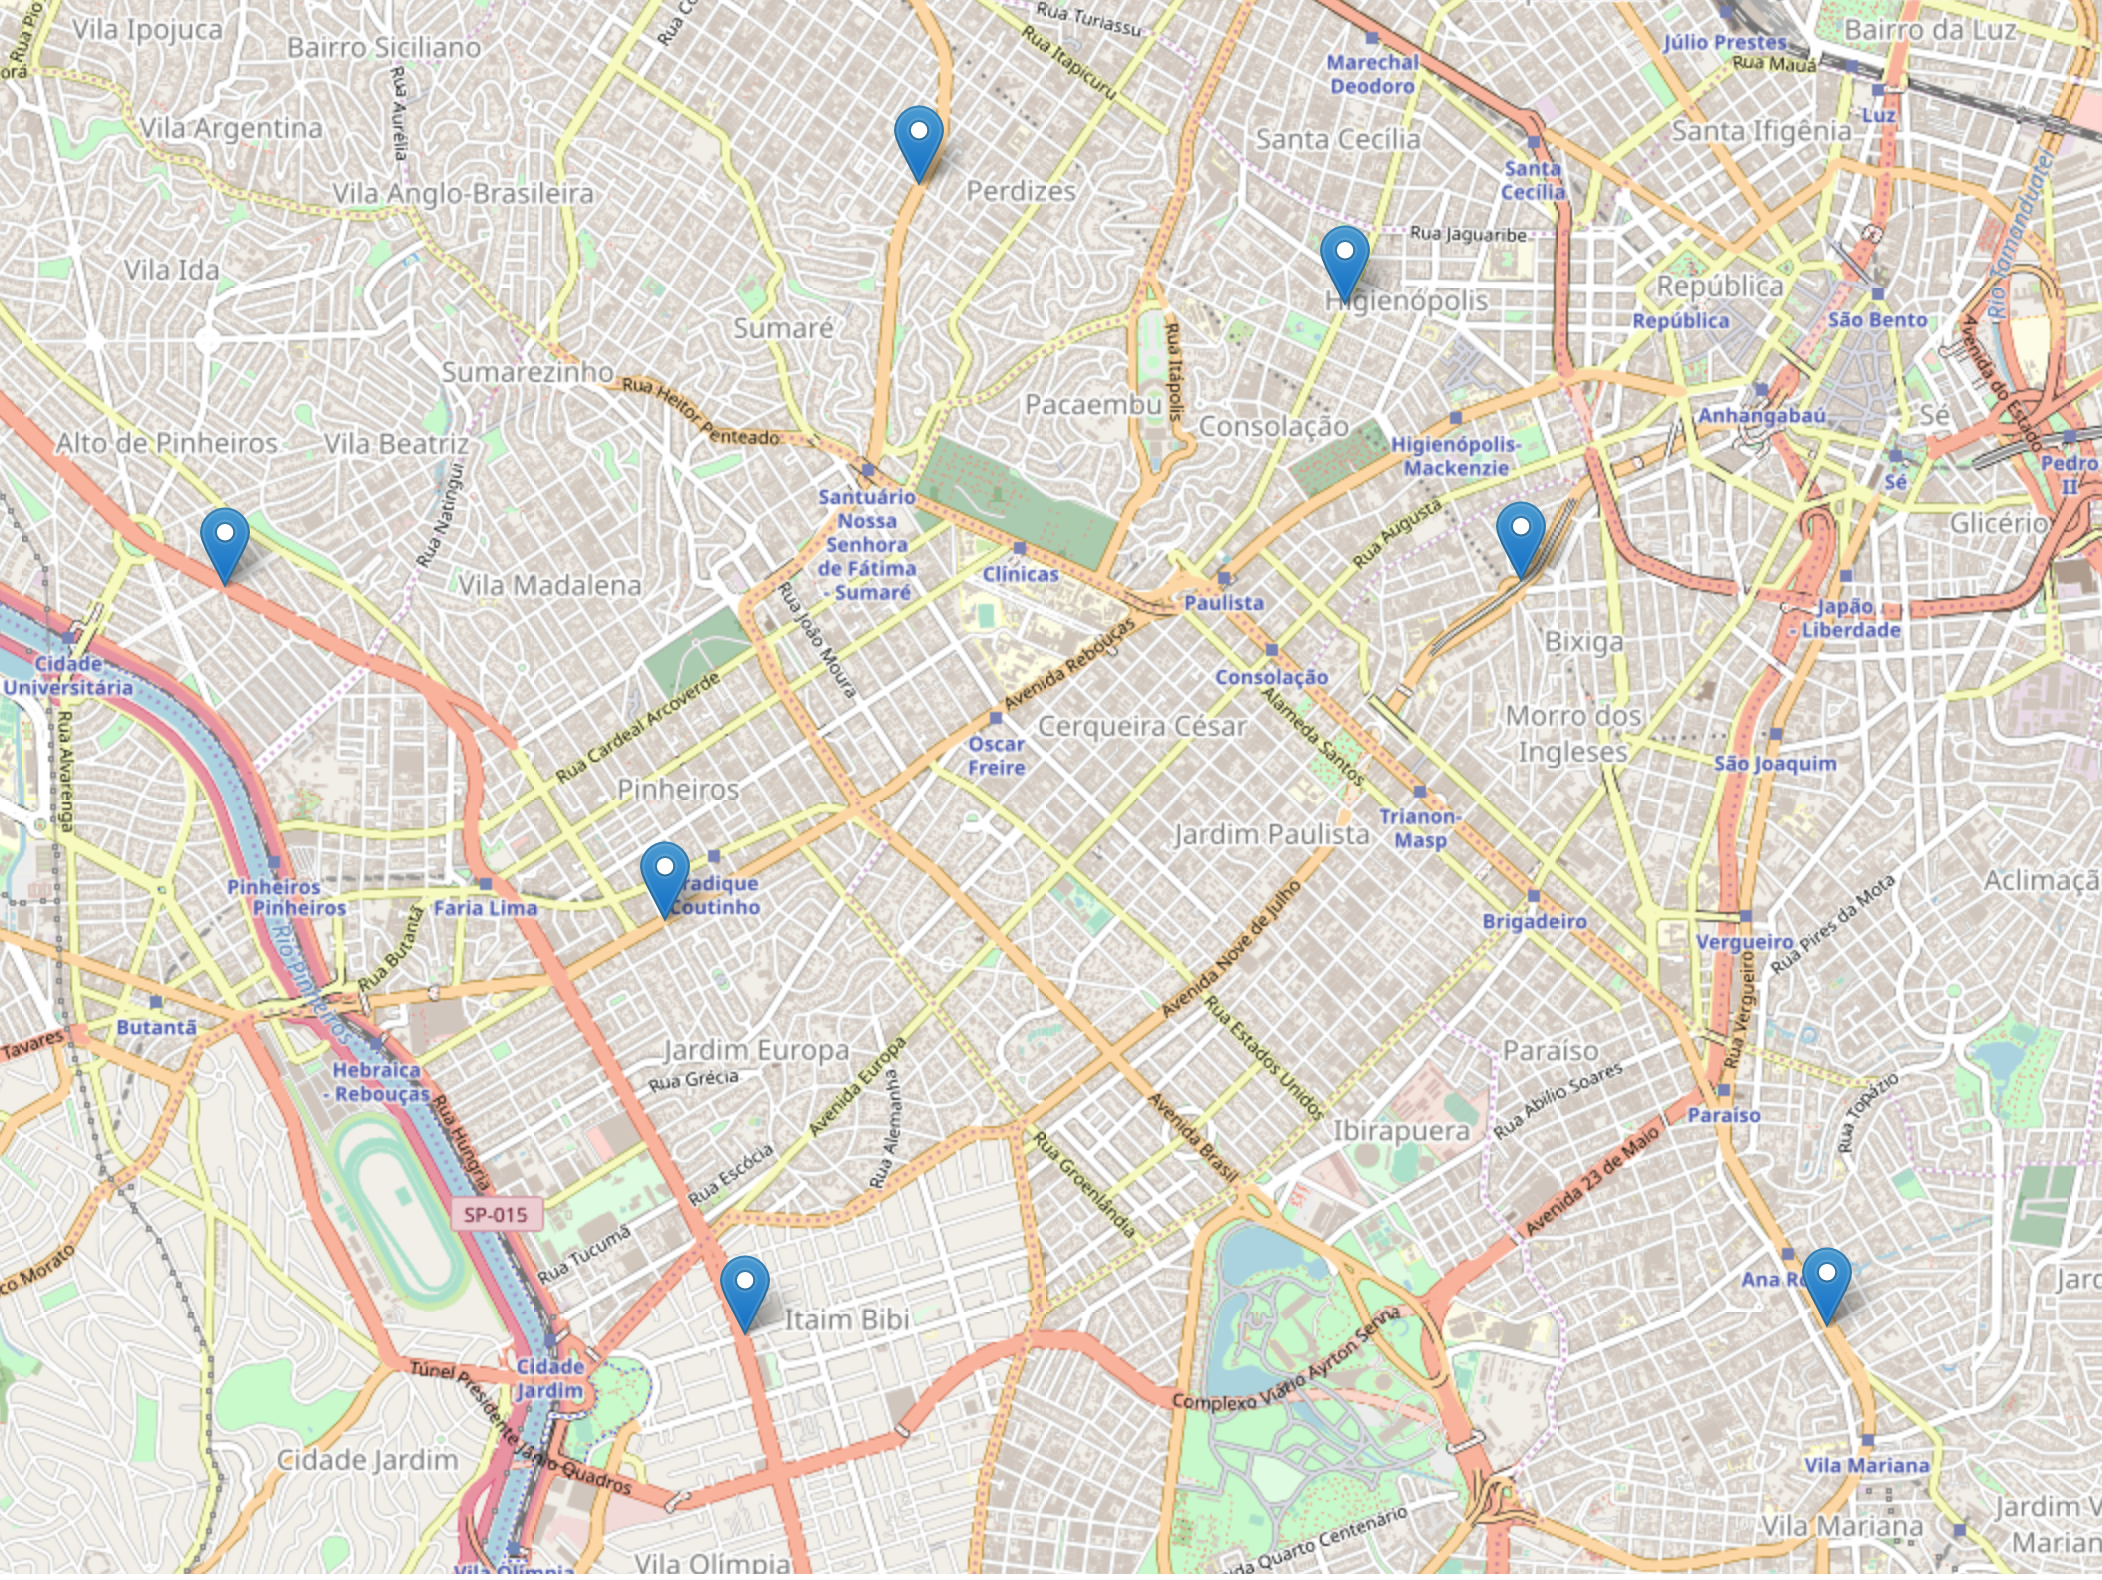
\includegraphics[width=.7\textwidth]{figuras/pmvs_locations.png}
	\caption{Posicionamento das PMVs no experimento de tráfego de carros inteligente.}
	\label{fig:pos_pmvs}
\end{figure}

E na Figura \ref{fig:eventos}, pode-se ver os trechos de vias que foram fechadas nas etapas 2 e 3 deste experimento.
No grafo do mapa viário da cidade gerado a partir do OpenStreet Maps, uma mesma via é formada de várias pequenas arestas (trechos de via).
Visando enfatizar um evento como um acidente de carro fatal ou um possível alagamento na região, fechamos um conglomerado de arestas nas proximidades das avenidas Rebouças e Paulista.

\begin{figure}[ht]
	\centering
	\includegraphics[width=.7\textwidth]{figuras/events_edges_map.png}
	\caption{Local dos eventos de fechamento de via no experimento de tráfego de carros inteligente.}
	\label{fig:eventos}
\end{figure}

Sabendo o local dos eventos de fechamento de vias e o posicionamento das PMVs, esperávamos que a notificação prévia dos motoristas sobre o acidente reduzisse a média do tempo de viagem dos motoristas
com relação a não existência das PMVs.
Consideramos que, pelo fato das avenidas Rebouças e Paulista serem bem movimentadas, muitas das viagens simuladas neste experimento passassem por aquele trecho. 
Contudo, a utilização das PMVs não deveria melhorar a média da duração das viagens em relação a etapa onde não acontece nenhum evento de fechamento de via.

As três etapas desse experimento foram realizadas novamente em dois \textit{laptops} com 8 CPUs virtuais (1.80 GHz) e 8 GB de memória RAM.
Mais uma vez, diferente do experimento apresentado na Seção \ref{sec:exp_smart_parking}, o foco desse experimento não é analisar o desempenho da plataforma, mas sim uma análise funcional. 
O passo a passo para execução desse experimento de validação foi o seguinte:

\begin{enumerate}
    \item Executar uma instância em modo de produção da plataforma InterSCity em um \textit{laptop}.

    \item Executar uma instância em modo de produção da simulador InterSCSimulator no outro \textit{laptop}.

    \item Configurar rede local entre os \textit{laptops}, conectados de maneira cabeada via ethernet.

    \item Realizar a simulação do cenário de tráfego de carros inteligente.

    \item Analizar os resultados obtidos ao final da simulação.
\end{enumerate}

A Figura \ref{fig:duracao_total}, apresenta o desvio padrão (no topo das barras) e a duração média das viagens de carro simuladas nas três etapas deste experimento.
No eixo Y, a duração é apresentada em segundos (ciclo de execução da simulação -- 1 ciclo = 1 segundo), e no eixo X os diferentes cenários utilizados em cada uma das 3 etapas.
Como podemos ver no gráfico apresentado, em geral, a média do tempo de duração das viagens não passou de 6 minutos.
Isso pode ter ocorrido pelo fato das viagens nessa região serem mais curtas, ou por não terem viagens suficientes para gerar congestionamentos, já que filtramos apenas as viagens que se iniciavam e
terminavam dentro do recorte do mapa utilizado.
Outro fator importante que nos chamou a atenção, foi a média da duração das viages da etapa 3, onde existem vias fechadas e o auxilio de PMVs, ser menor do que da etapa 1, onde não existe qualquer
incidente.
Após analisar os dados, percebemos que ao recalcular a rota quando deparado de uma PMV, os carros se distribuíam de uma melhor forma pela malha viária do cenário utilizado pelo experimento, com isso,
evitavam congestionamentos que ocorriam anteriormente.
Sendo isso um alvo de possível melhoria no simulador, já que o mesmo ao criar o ator, calcula e utiliza apenas um dos menores caminhos entre a origem e destino do carro, podendo essa rota coincidir entre
múltiplos atores com origem e destinos similares, assim, deixando outros caminhos mais curtos inutilizados.
Todavia, como esperado, a etapa 2, onde temos fechamento de vias mas não temos PMVs, teve a maior média de duração das viagens.

\begin{figure}[ht]
	\centering
	\includegraphics[width=.8\textwidth]{figuras/duracao_total.png}
	\caption{Média da duração das viagens de carros no experimento.}
	\label{fig:duracao_total}
\end{figure}

Para garantirmos uma melhor acurácia na análise dos resultados obtidos, filtramos apenas as viagens que foram influencidas de alguma forma pelo fechamento de vias e/ou PMVs.
Isso porque percebemos a existência de viagens que não eram modificadas em nenhuma das etapas do experimento, ou seja, a sua duração era sempre a mesma.
Na Figura \ref{fig:duracao_filtered}, apresentamos o mesmo gráfico discutido anteriormente, só que incluindo apenas as viagens que foram afetadas.
Agora analisando o gráfico com as viagens afetadas, obtivemos o resultado esperado no início do experimento.
A etapa 1, onde não há vias fechadas, teve o menor tempo médio de duração de viagens, sendo esse o nosso limite inferior.
A etapa 2, onde vias foram fechadas, o pior tempo médio de viagem foi obtido, sendo o limite superior.
E a etapa 3, onde introduzimos as PMVs para auxiliar os motoristas na decisão da melhor rota a seguir, apresentou um tempo médio de viagem ligeiramente menor do que a etapa 2 e maior do que a etapa 1.

\begin{figure}[ht]
	\centering
	\includegraphics[width=.8\textwidth]{figuras/duracao_filtered.png}
	\caption{Média da duração das viagens de carros afetadas por fechamento de vias e/ou PMVs no experimento.}
	\label{fig:duracao_filtered}
\end{figure}

Contudo, a melhora de aproximadamente 5\% na média do tempo de duração da viagem da etapa 3 com relação a etapa 2 não foi um resultado expressivo.
Avaliamos que alguns fatores podem ter influenciado nesse resultado, sendo a maioria deles voltado para os dados utilizados para a definicação do cenário de simulação deste experimento.
O posicionamento das PMVs pode não ter sido o ideal, já que não foi realizada uma análise prévia de onde passariam a maior parte dos carros.
O conjunto de viagens simulados após recortar o mapa da cidade de São Paulo pode não ter sido representativo, a decisão de reduzir o mapa para facilitar a visualização do impacto do fechamento de vias
e PMVs pode não ter sido boa ideia.
Além disso, os resultados obtidos podem ter sido influenciados devido a infraestrutura simples utilizada com apenas dois \textit{laptops}.


\section{Análise Crítica}

% Melhorias, o que fucionou, o que não funcionou

Após a realização dos dois estudos de caso apresentados neste capítulo, foi possível perceber que as implementações da solução proposta no Capítulo \ref{cap:proposta} são funcionais e nos permitiram realizar
diferentes experimentos utilizando um ambiente simulado de uma cidade, podendo substituir \textit{testbeds} reais e aumentando a escala dos experimentos.

Um ponto importante para a realização de experimentos, e ainda mais envolvendo múltiplas ferramentas, é a automatização desse processo.
Tal automatização facilita a execução de várias rodadas do experimento e a reprodução do trabalho por terceiros.
Neste trabalho, acreditamos que ambos os estudos de caso foram devidamente automatizados e documentados, favorecendo a continuidade do trabalho.

No primeiro estudo de caso conseguimos evidenciar a escalabilidade horizontal da plataforma InterSCity.
Várias melhorias foram realizadas e gargalos solucionados, o que nos demonstrou a extrema importância da realização desse tipo de experimento durante o ciclo de desenvolvimento de plataformas de Cidades
Inteligentes.
Já no segundo estudo de caso, demonstramos a viabilidade da atuação em tempo de execução em um ambiente simulado, sendo esse um trabalho pioneiro na área de Cidades Inteligentes.
 
Contudo, como o foco principal do trabalho é prover uma solução de ambiente simulado para a realização de experimentos em plataformas de Cidade Inteligentes, acreditamos que algumas das análises
apresentadas nos estudos de caso poderiam ser melhoradas.
Ademais, especialmente no segundo estudo de caso, algumas decisões iniciais do experimento poderiam ser otimizadas, como o posicionamento das PMVs baseado em uma análise mais profunda da movimentação
dos carros nas viagens selecionadas para o experimento, o que prejudicou os resultados obtidos.
A utilização de \textit{laptops} para a execução do segundo experimento também contribuiu para o resultado final abaixo do esperado, tendo em vista que esse tipo de experimento requer muitos recursos
computacionais.

Em suma, os estudos de caso foram satifatórios, já que foi possível validar a proposta de solução em dois cenários de Cidades Inteligentes distintos, exercitando as principais funcionalidades que
um ambiente de experimentação simulado deve possuir.


